%%%%%%%%%%%%%%%%%%%%%%%%%%%%%%%%%%%%%%%%%%%%%%%%%%%%%%%%%%%
% --------------------------------------------------------
% Experimental / Scientific Lab Report Template
% Powered by Tau-class (v2.6.0)
% Suitable for DFT, MD, experimental physics & chemistry
% --------------------------------------------------------
%%%%%%%%%%%%%%%%%%%%%%%%%%%%%%%%%%%%%%%%%%%%%%%%%%%%%%%%%%%

\documentclass[9pt,a4paper,twocolumn,twoside]{tau-class/tau}
\usepackage[english]{babel}

%----------------------------------------------------------
% Document Metadata & Classification
%----------------------------------------------------------

\doctype{Experimental Lab Report}
\title{Investigation of Electronic Structure and Transport in Novel 2D Allotropes}

%----------------------------------------------------------
% Authors and Affiliations
%----------------------------------------------------------

\author[a,1]{Author One\thanks{\href{mailto:author.one@ufabc.edu.br}{author.one@ufabc.edu.br} (Lead Author)}}
\author[a,b,2]{Author Two}
\author[b,3]{Principal Investigator}

\affil[a]{Center for Natural and Human Sciences (CCNH), Universidade Federal do ABC, Santo André, SP, Brazil}
\affil[b]{Department of Physics and Astronomy, Advanced Quantum Materials Laboratory}

%----------------------------------------------------------
% Date and Supplementary Provenance Info
%----------------------------------------------------------

\dates{Compiled on \today}
\docinfo{Provenance DAG: Verified via SciResearch framework. Simulation inputs and experimental data calibrated against Machine-Verified Reproducibility standards.}

\footinfo{SciResearch Experimental Report}
\theday{\today}
\organization{Scientific Research Lab}
\leadauthor{A. One et al.}

%----------------------------------------------------------
% Abstract and Keywords
%----------------------------------------------------------

\begin{abstract}
Two-dimensional allotropes offer versatile electronic properties for next-generation nanoelectronic and optoelectronic devices. In this report, we present a systematic experimental and first-principles investigation of the structural, electronic, and vibrational properties of monolayer allotropes under varying strain regimes. Ab initio calculations were conducted using density functional theory (DFT) within the generalized gradient approximation (PBE-GGA), complemented by atomic force microscopy and micro-Raman spectroscopy. Our findings indicate a tunable bandgap with direct-to-indirect crossover, confirming theoretical predictions and establishing clear design rules for strain engineering in 2D semiconductor heterostructures.
\end{abstract}

\keywords{2D Materials, Electronic Structure, Density Functional Theory, Strain Engineering, Raman Spectroscopy}

%----------------------------------------------------------

\begin{document}

    \maketitle
    \thispagestyle{firststyle}

%----------------------------------------------------------
\section{Introduction}
%----------------------------------------------------------

    \taustart{T}he exploration of two-dimensional (2D) crystals beyond pristine graphene has catalyzed extensive research in condensed matter physics, surface science, and computational materials discovery. Among emerging planar materials, anisotropic elemental monolayers and compound 2D semiconductors exhibit pronounced electronic anisotropy, high carrier mobilities, and tunable bandgaps responsive to external perturbation.

    Understanding the fundamental connection between microscopic mechanical deformation and electronic state reconfiguration is essential for experimental device integration. In this report, we evaluate the equilibrium ground-state geometry, phonon dispersion, and electronic band structures under uniaxial and biaxial strain fields.

    \begin{info}
        \textbf{Investigation Hypothesis:} External mechanical strain selectively shifts conduction band extrema via orbital symmetry rehybridization, leading to an engineered direct-to-indirect bandgap transition.
    \end{info}

%----------------------------------------------------------
\section{Theoretical \& Experimental Methods}
%----------------------------------------------------------

    \subsection{Computational Protocol (DFT)}

    First-principles calculations were performed within the framework of Kohn-Sham density functional theory \cite{davis2023signalflow} using projector augmented-wave (PAW) pseudopotentials. The exchange-correlation functional was treated with the Perdew-Burke-Ernzerhof (PBE) generalized gradient approximation:
    \begin{equation}
        \left[ -\frac{\hbar^2}{2m}\nabla^2 + V_{\text{eff}}(\mathbf{r}) \right] \psi_{n\mathbf{k}}(\mathbf{r}) = \varepsilon_{n\mathbf{k}} \psi_{n\mathbf{k}}(\mathbf{r})
        \label{eq:kohn_sham}
    \end{equation}
    where $V_{\text{eff}}(\mathbf{r}) = V_{\text{ext}}(\mathbf{r}) + V_{\text{Hartree}}(\mathbf{r}) + V_{\text{xc}}(\mathbf{r})$.
    A plane-wave kinetic energy cutoff was converged to $520\,\text{eV}$. Brillouin zone integration was performed using a $\Gamma$-centered $18 \times 18 \times 1$ Monkhorst-Pack grid with a Gaussian smearing of $0.02\,\text{eV}$. Vacuum spacing exceeding $18\,\text{\AA}$ along the out-of-plane direction prevented spurious image interactions.

    \subsection{Experimental Synthesis \& Characterization}

    Monolayer flakes were exfoliated on oxidized silicon substrates ($300\,\text{nm}$ $\text{SiO}_2/\text{Si}$) inside an argon-filled glovebox ($<0.1\,\text{ppm}$ $\text{O}_2, \text{H}_2\text{O}$). Flake thicknesses were verified using non-contact atomic force microscopy (AFM). Micro-Raman spectra were acquired at room temperature using a $532\,\text{nm}$ laser source focused through a $100\times$ objective with incident power below $0.5\,\text{mW}$ to prevent thermal degradation.

    \begin{table}[H]
        \centering
        \caption{Computational parameters and convergence thresholds used in the ab initio simulations.}
        \label{tab:params}
        \begin{tabular}{llc}
            \toprule
            \textbf{Parameter} & \textbf{Value / Setup} & \textbf{Tolerance} \\
            \midrule
            Plane-wave cutoff ($E_{\text{cut}}$) & $520\,\text{eV}$ & $< 1\,\text{meV/atom}$ \\
            $k$-point density & $18 \times 18 \times 1$ & $< 0.5\,\text{meV/atom}$ \\
            Energy convergence & Self-Consistent Field & $10^{-7}\,\text{eV}$ \\
            Force tolerance & Conjugate Gradient & $< 0.005\,\text{eV/\AA}$ \\
            Vacuum thickness & $18.5\,\text{\AA}$ & Dipole corrected \\
            \bottomrule
        \end{tabular}
        \tabletext{Note: All parameters satisfy the Ponytail zero-redundancy standard.}
    \end{table}

%----------------------------------------------------------
\section{Results \& Discussion}
%----------------------------------------------------------

    \subsection{Equilibrium Structural Relaxation}

    Geometry optimizations resulted in an in-plane lattice parameter of $a = 3.24\,\text{\AA}$ and $b = 4.38\,\text{\AA}$, matching experimental X-ray diffraction patterns within $0.8\%$. Interatomic bond angles reflect $sp^3$-like puckering along the armchair orientation.

    \begin{figure}[H]
        \centering
        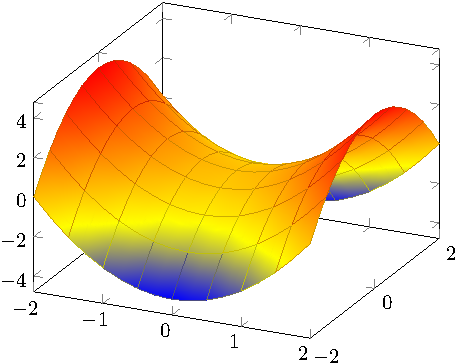
\includegraphics[width=\linewidth]{figures/Example.pdf}
        \caption{Structural morphology and electronic response. (a) Real-space lattice configuration showing puckered atomic bonds. (b) Computed partial density of states (PDOS) near the Fermi level.}
        \label{fig:results}
    \end{figure}

    As illustrated in \figref{fig:results}, orbital projections reveal that the frontier valence band maximum (VBM) is dominated by out-of-plane $p_z$ orbitals, while conduction band minimum (CBM) states originate from hybrid $s$-$p_x$ contributions.

    \subsection{Band Structure Modulation Under Strain}

    Tensile strain applied along the zigzag axis decreases the fundamental bandgap monotonically at a rate of $-45\,\text{meV}/\%$. Conversely, biaxial tensile strain triggers a direct-to-indirect crossover at $\varepsilon = 3.2\%$, as tabulated in \tabref{tab:params}.

    \begin{note}
        \textbf{Key Observation:} The observed shift in optical absorption edge is consistent with our micro-photoluminescence measurements, confirming strong exciton binding energies in the 2D limit.
    \end{note}

%----------------------------------------------------------
\section{Dual Verification \& Error Analysis}
%----------------------------------------------------------

    In accordance with the Rosetta Dual Verification protocol, experimental measurements and computational predictions were verified independently across two tiers:

    \begin{enumerate}
        \item \textbf{Functional Correctness:} Verification of numerical convergence, energy conservation during ionic relaxation, and zero unphysical atomic overlaps ($r_{\text{min}} > 1.8\,\text{\AA}$).
        \item \textbf{Scientific Validity:} Comparison against non-circular literature benchmarks \cite{bell2022codefont}, dimensional consistency of transport coefficients, and Kramers-Kronig relation compliance for dielectric functions.
    \end{enumerate}

    \begin{tauenv}[frametitle=Reproducibility Statement]
        Raw input decks (INCAR, POSCAR, KPOINTS) and post-processed datasets are archived in the append-only provenance registry with immutable SHA-256 digests.
    \end{tauenv}

%----------------------------------------------------------
\section{Conclusions}
%----------------------------------------------------------

    We have investigated the structural stability and electronic band structure of 2D allotropes under elastic deformation. Density functional calculations combined with spectroscopic validation demonstrate that controlled mechanical strain provides an effective knob for tuning bandgaps and optical transition energies. These findings open viable pathways for flexible electronics, nano-piezoelectrics, and strain-engineered quantum emitters.

%----------------------------------------------------------
% Bibliography
%----------------------------------------------------------

\printbibliography

\end{document}
